\section{Arquitectura}

En esta secci\'on presentaremos y analizaremos la arquitectura pensada para resolver el trabajo, as\'i como las t\'acticas utilizadas para asegurar los atributos de calidad que se mencionaron anteriormente.

\subsection{Comunicaci\'on con Drones}

Para el monitoreo de las plantaciones se utilizar\'an drones que tomar\'an fotograf\'ias y luego ser\'an analizadas para recaudar la informaci\'on necesaria.  Para esto, contamos con un componente dedicado a la comunicaci\'on con las interfaces de manejo de drones que nos provee el Ministerio y la empresa privada. Se utilizar\'a por default el sistema de drones estatales, en caso de no responder a los pedidos, se pasara a utilizar el sistema privado.

A medida que se reciben las im\'agenes, se pasan utilizando una cola al geolocalizador que se encarga de identificar las plantaciones: analizando las im\'agenes y usando la informaci\'on del repositorio de geolocalizaciones. Este componente se encarga tambi\'en de descartar las im\'agenes err\'oneas que no permiten un an\'alisis.

El repositorio contiene informaci\'on ingresada por los usuarios sobre la localizaci\'on de las plantaciones, as\'i como su estado. Esta informaci\'on se utiliza para comparar con el an\'alisis que haga el geolocalizador y poder verificar de qu\'e plantaci\'on se trata.

Una vez tageada la imagen se env\'ia a los analizadores que trabajan en paralelo para reconocer la T\textdegree, el estado del suelo y la salinidad del agua. Luego de esto se procede a mergear los resultados y guardarlos en el repo de informaci\'on.



\begin{figure}[h!]
  \centering
  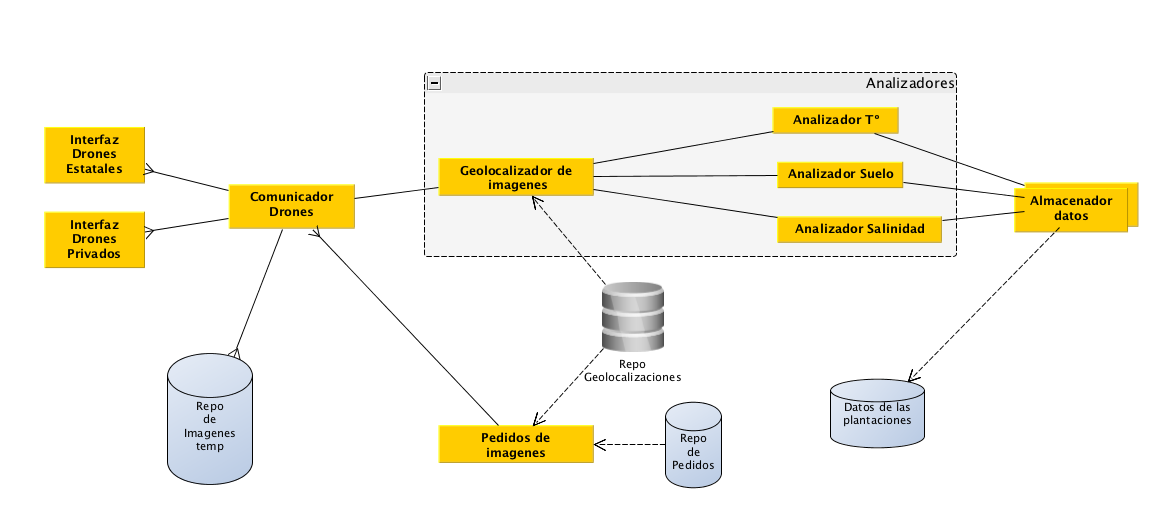
\includegraphics[width=1\textwidth]{./images/arq_drones.png}
  \caption{Arquitectura de comunicaci\'on con drones y procesamiento de im\'agenes}
  \label{fig:clases4}
\end{figure}

\begin{figure}[h!]
  \centering
  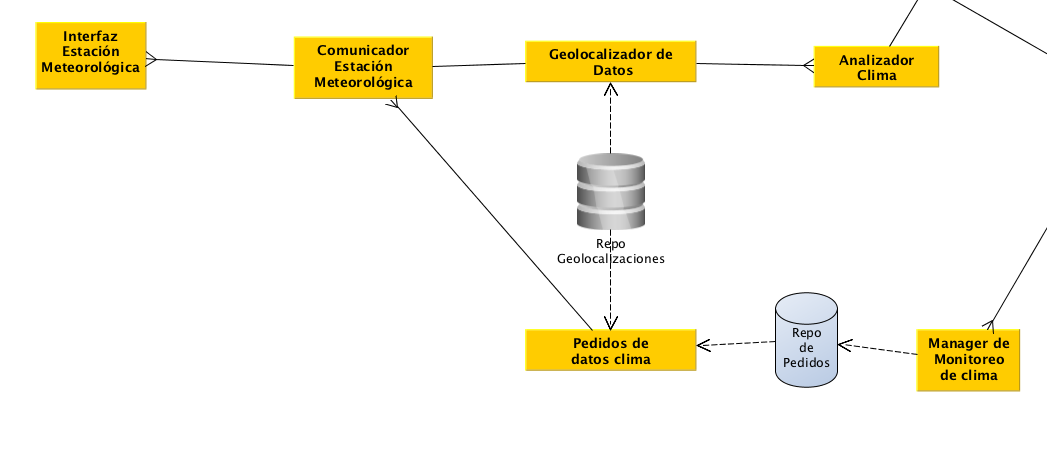
\includegraphics[width=1\textwidth]{./images/arq_clima.png}
  \caption{Arquitectura de comunicaci\'on con estaciones meteorol\'ogicas y procesamiento de datos}
  \label{fig:clases4}
\end{figure}

\begin{figure}[h!]
  \centering
  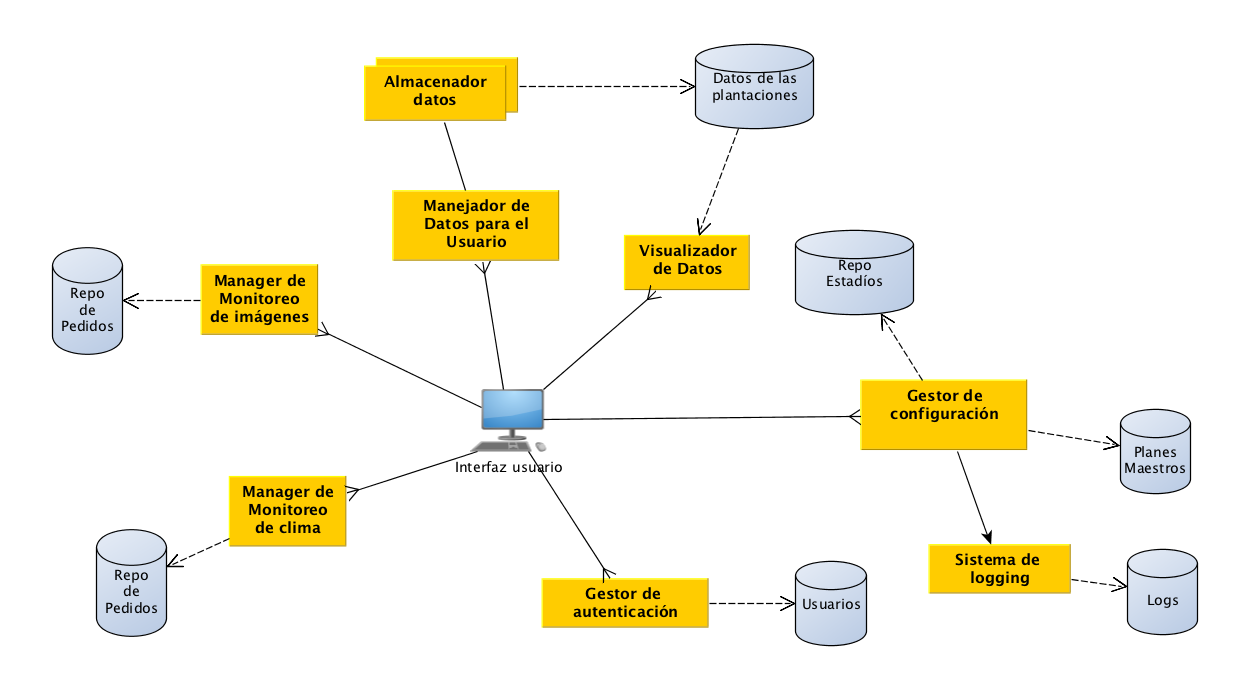
\includegraphics[width=0.4\textwidth]{./images/arq_interfazusuario.png}
  \caption{Arquitectura de comunicaci\'on con la interfaz de usuario}
  \label{fig:clases4}
\end{figure}

\begin{figure}[h!]
  \centering
  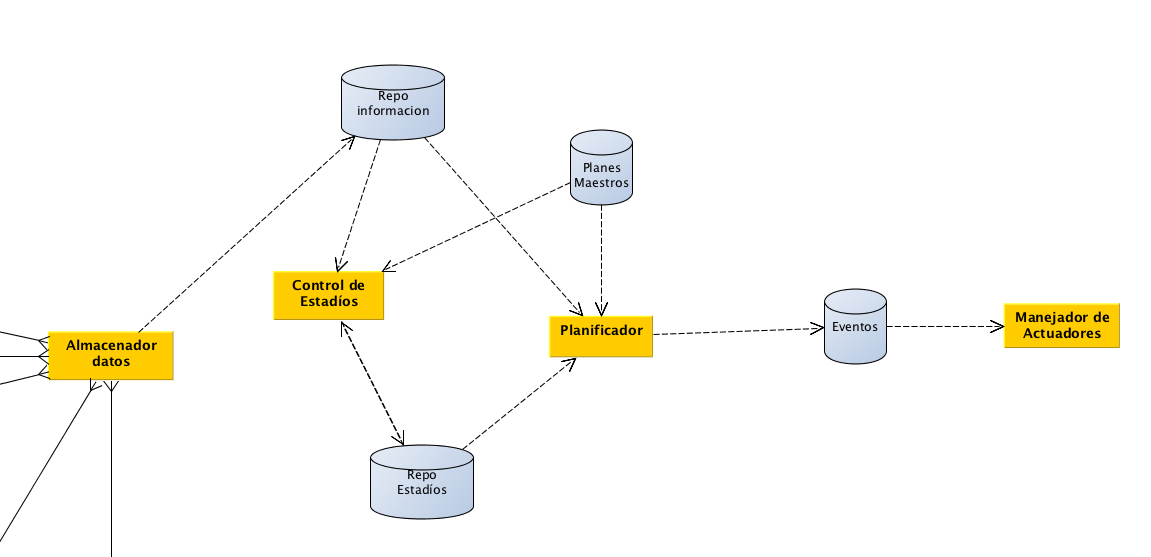
\includegraphics[width=1\textwidth]{./images/arq_plan.png}
  \caption{Arquitectura de planificaci\'on de eventos}
  \label{fig:clases4}
\end{figure}